\chapter{Исследовательская часть}

Цель исследования — классифицировать данные из mnist dataset, используя нейросетевой подход с ReLU функцией активации и KL Divergence функцией потерь.

\section{Оборудование}

Характеритстики ноутбука:
\begin{itemize}
	\item процессор intel-core i5-12500H \cite{lib:intel}
	\item ОЗУ 16 Гб DDR4 
	\item ОС Windows 11 \cite{lib:windows}
\end{itemize}

\section{Результаты исследования}

\begin{figure}[H]
    \centering
    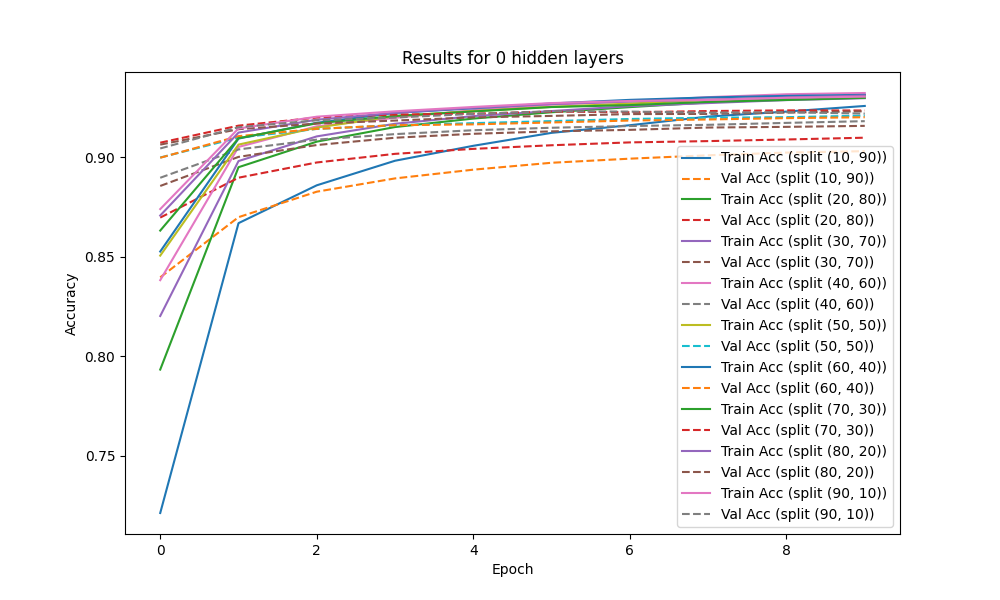
\includegraphics[width=1\linewidth]{C:/MGTU/baseAI/lr5/bag/report/images/Results for 0 hidden layers.png}
    \caption{Влияние соотношения обучающей и валидационной выборки на обучение модели без скрытых слоёв}
\end{figure}

\begin{figure}[H]
    \centering
    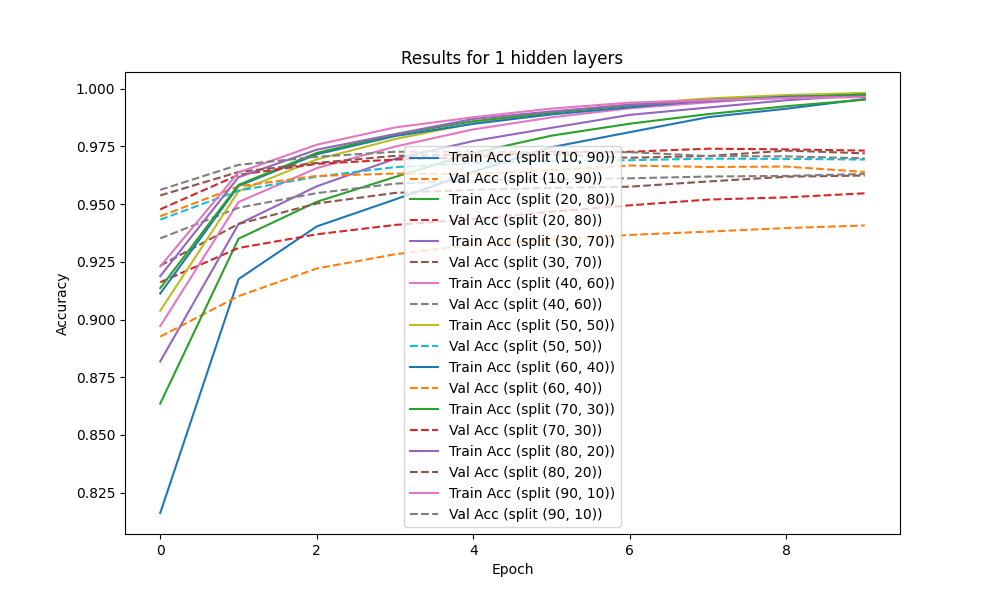
\includegraphics[width=1\linewidth]{C:/MGTU/baseAI/lr5/bag/report/images/Results for 1 hidden layers.png}
    \caption{Влияние соотношения обучающей и валидационной выборки на обучение модели с 1 скрытым слоем}
\end{figure}

\begin{figure}[H]
    \centering
    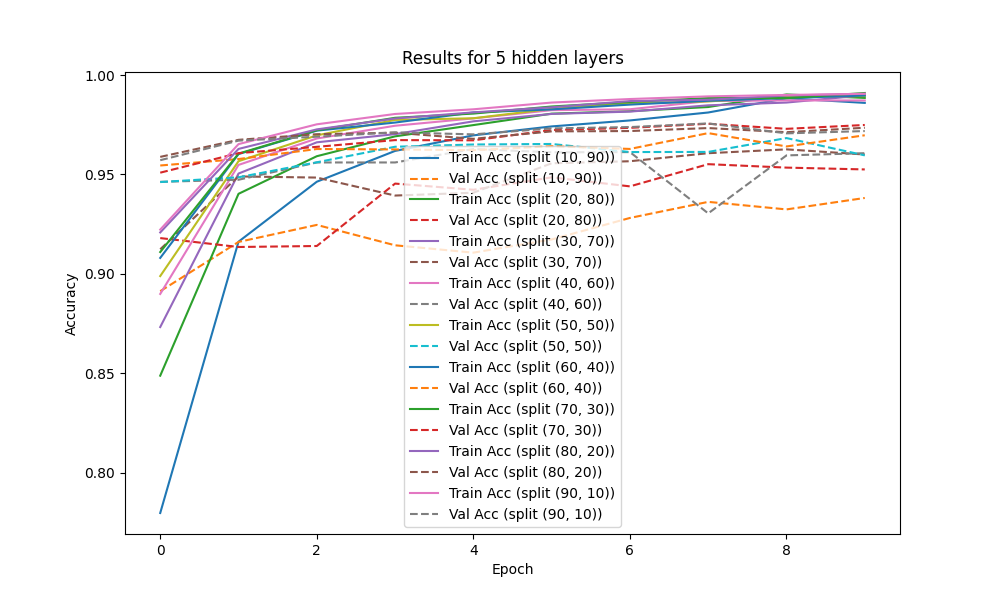
\includegraphics[width=1\linewidth]{C:/MGTU/baseAI/lr5/bag/report/images/Results for 5 hidden layers.png}
    \caption{Влияние соотношения обучающей и валидационной выборки на обучение модели с 5 скрытыми слоями}
\end{figure}

\begin{table}[H]
    \centering
    \caption{Размер выборки по Чебышёву для разных разбиений трен./валид. выборки}
    \begin{tabular}{|c|c|}
    \hline
    Соотношение трен./валид. выборки & Чебышёв Размер \\
    \hline
    (10, 90) & 48 \\
    (20, 80) & 42 \\
    (30, 70) & 46 \\
    (40, 60) & 42 \\
    (50, 50) & 45 \\
    (60, 40) & 44 \\
    (70, 30) & 47 \\
    (80, 20) & 44 \\
    (90, 10) & 45 \\
    \hline
    \end{tabular}
\end{table}

\begin{table}[h]
    \centering
    \caption{Результаты тестирования для разных разбиений и количества скрытых слоёв}
    \begin{tabular}{|c|c|c|c|}
    \hline
    Соотношение трен./валид. выборки & Скрытые слои & Потери & Точность \\
    \hline
    (10, 90) & 0 & 0.3216 & 0.9096 \\
    (10, 90) & 1 & 0.1931 & 0.9430 \\
    (10, 90) & 5 & 0.2894 & 0.9429 \\
    \hline
    (20, 80) & 0 & 0.2943 & 0.9172 \\
    (20, 80) & 1 & 0.1499 & 0.9568 \\
    (20, 80) & 5 & 0.2032 & 0.9521 \\
    \hline
    (30, 70) & 0 & 0.2860 & 0.9213 \\
    (30, 70) & 1 & 0.1250 & 0.9673 \\
    (30, 70) & 5 & 0.1629 & 0.9622 \\
    \hline
    (40, 60) & 0 & 0.2777 & 0.9237 \\
    (40, 60) & 1 & 0.1230 & 0.9665 \\
    (40, 60) & 5 & 0.1497 & 0.9649 \\
    \hline
    (50, 50) & 0 & 0.2716 & 0.9234 \\
    (50, 50) & 1 & 0.1175 & 0.9712 \\
    (50, 50) & 5 & 0.1991 & 0.9576 \\
    \hline
    (60, 40) & 0 & 0.2750 & 0.9241 \\
    (60, 40) & 1 & 0.1270 & 0.9644 \\
    (60, 40) & 5 & 0.1325 & 0.9701 \\
    \hline
    (70, 30) & 0 & 0.2704 & 0.9249 \\
    (70, 30) & 1 & 0.0997 & 0.9752 \\
    (70, 30) & 5 & 0.1270 & 0.9742 \\
    \hline
    (80, 20) & 0 & 0.2700 & 0.9253 \\
    (80, 20) & 1 & 0.1064 & 0.9728 \\
    (80, 20) & 5 & 0.1070 & 0.9764 \\
    \hline
    (90, 10) & 0 & 0.2681 & 0.9285 \\
    (90, 10) & 1 & 0.1084 & 0.9721 \\
    (90, 10) & 5 & 0.1214 & 0.9740 \\
    \hline
    \end{tabular}
\end{table}

\section*{Вывод}

Проведённые исселодвания показали, что увеличение количества скрытых слоёв улучшает точность и снижает потери на тестовой выборке, 
однако прирост качества становится незначительным при переходе от одного скрытого слоя к пяти. 
Оптимальной в данном случае можно считать архитектуру с одним скрытым слоем, которая обеспечивает баланс между качеством и сложностью модели.

Кроме того, распределение данных между обучающей и валидационной выборками оказывает влияние на результаты. 
Более высокие значения точности достигаются при большем объёме данных для обучения (Split: 90/10 и 80/20).

\clearpage
